\documentclass[11pt,letterpaper]{article}

\usepackage[letterpaper,margin=0.8in,nohead]{geometry}

\usepackage[colorlinks]{hyperref}
\usepackage{url}
\usepackage{breakurl}

\hypersetup{
	colorlinks,
	linkcolor={red},
	citecolor={red},
	urlcolor={blue}
}

\usepackage{verbatim}
\usepackage{fancyvrb}
\usepackage{scrextend}
\usepackage{enumitem}
\usepackage{url}
\usepackage{tabularx}
\usepackage{float}

\usepackage{caption}
\usepackage{graphicx}
\usepackage{subcaption}

\usepackage{changepage}   % for the adjustwidth environment

\newenvironment{answer}{\em \color{blue} \begin{adjustwidth}{1cm}{1cm}}{\end{adjustwidth}}

% math
\usepackage{amsthm,amsmath}
\usepackage{amsfonts}

\newcommand{\mc}[1]{\mathcal{#1}}	% Mechanisms / Algorithms
\newcommand{\rv}[1]{\mathbf{#1}}    % Random variable

\newcommand{\pr}[1]{\mathrm{Pr}\{#1\}} % Probability

\newtheorem{corollary}{\bf Corollary}%[theorem]
\newtheorem{lemma}{\bf Lemma}%[theorem]
\newtheorem{definition}{\bf Definition}%[section]

\newtheorem{observation}{\bf Observation}%[theorem]

% load cleveref last!
\usepackage[capitalise]{cleveref}


\begin{document}
	
	\title{EN4720: Security in Cyber-Physical Systems \\ Exercise --- Infrastructure Security}
	
	%% This is an individual assignment!!
	%% TODO: put your name and index number here here!
	\author{ \textcolor{blue}{Name: Thalagala B. P.} \\ \textcolor{blue}{Index No: 180631J}}
	
	\maketitle
	
	\begin{center}
		\color{red}\bf This is an individual exercise! \\ Due Date: 20 June 2023 by 11.59 PM
	\end{center}
	
	% \begin{center}
		%     \small Content adopted from the Udacity Security Engineer Nano-Degree
		% \end{center}
	
	\vspace{1in}
	
	This exercise has to be carried out using a Linux-based PC/virtual machine. Read all the instructions and questions before attempting the exercise. Add answers under each question and submit the resulting PDF.
	
	
	\newpage
	\section*{Section 1}
	
	In this section, you will implement Firewall rules using \textbf{iptables} and \textbf{ufw} Linux commands. Moreover, you will scan network ports of a remote device using \textbf{nmap} Linux command.  
	
	For all the questions in this section, add a screenshot of the terminal (including all the commands you ran to perform the task) unless specified otherwise. The evaluator should be able to see each step that you followed to perform each task. In all screenshots, the areas marked (which are unique to your terminal display) in Figure 1 (the sample answer to Question 1) must be visible.
	
	\begin{enumerate}
		
		\item View the currently logged in user.
		
		\begin{figure}[H]
			\centering
			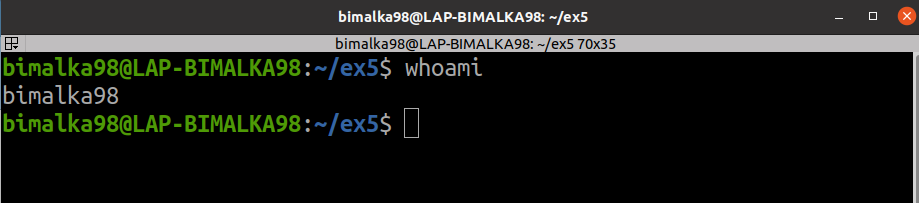
\includegraphics[width=0.65\columnwidth]{images/part1/1.png}
			\caption{Currently logged-in user} \label{fig:1}
		\end{figure}
		
		\subsubsection*{Creating Firewall Rules with iptables}
		
		\item Use \texttt{dpkg -l \textbar \ grep iptables} command to check whether iptables is installed on your system. If it does not existing in your system, install it by running \texttt{sudo apt-get install iptables}.
		
		\begin{answer}
			\begin{figure}[H]
				\centering
				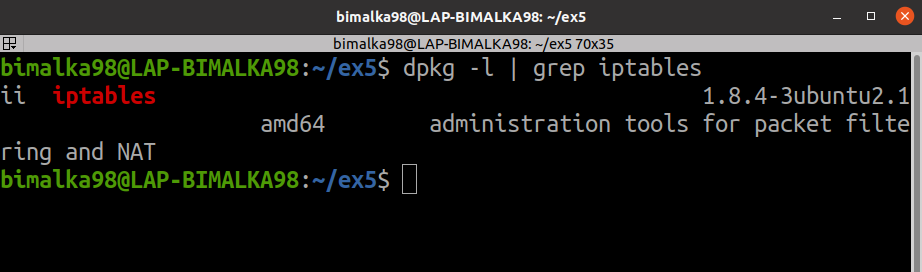
\includegraphics[width=0.65\columnwidth]{images/part1/2.png}
				\caption{Checking whether {\tt iptables} is installed on the system}
			\end{figure}
		\end{answer}
		
		\item Check all available iptables rules in your system using the command \texttt{/sbin/iptables -n -L }.
		
		\begin{answer}
			\begin{figure}[H]
				\centering
				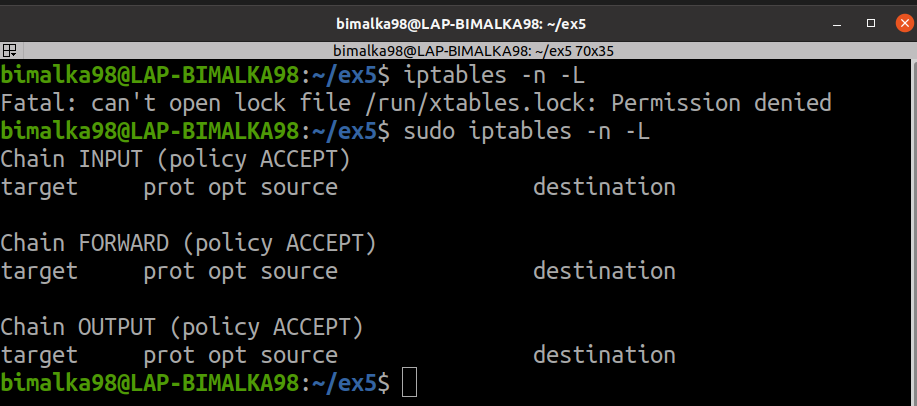
\includegraphics[width=0.65\columnwidth]{images/part1/3.png}
				\caption{Checking all available {\tt iptables} rules}
			\end{figure}
		\end{answer}
		
		\item Save all available iptables rules to a file named \textbf{iptablesRule.v4} using \texttt{iptables-save} command.
		
		\begin{answer}
			\begin{figure}[H]
				\centering
				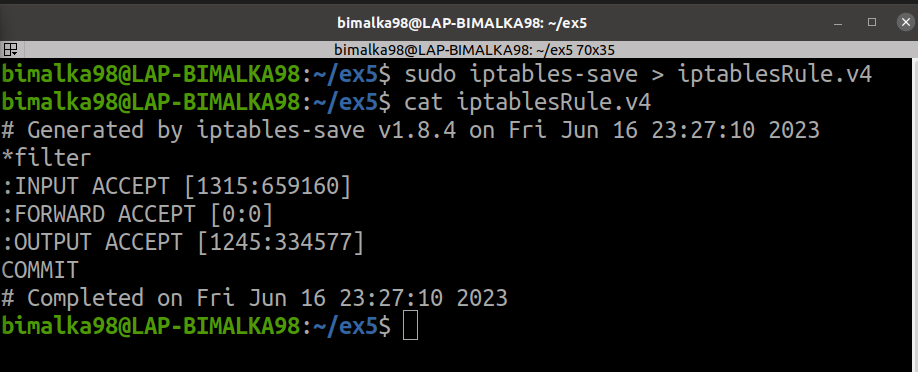
\includegraphics[width=0.65\columnwidth]{images/part1/4.png}
				\caption{Saving all available {\tt iptables} rules}
			\end{figure}
		\end{answer}
		
		\item Flush all the iptables rules that exist in your system and set a default policy to drop packets.
		\begin{answer}
			\begin{figure}[H]
				\centering
				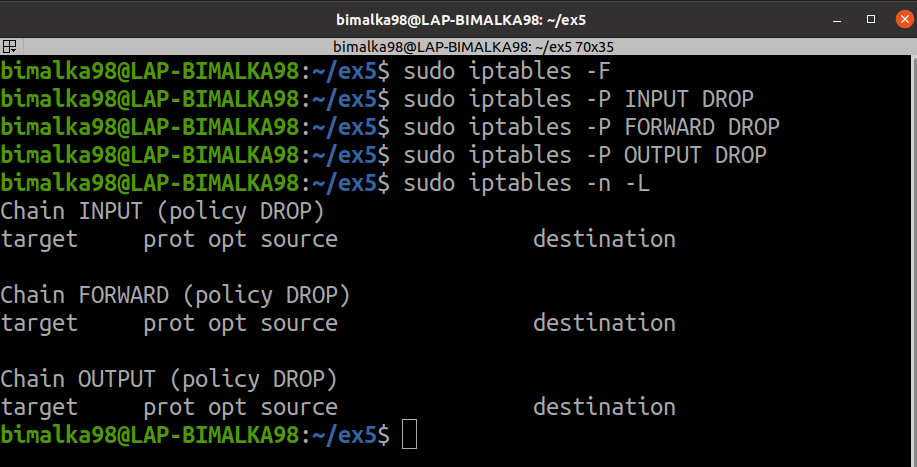
\includegraphics[width=0.65\columnwidth]{images/part1/5.png}
				\caption{Flushing all the rules and setting a default policy to drop packets}
			\end{figure}
		\end{answer}
		
		\item Set iptables rules to permit input and output DNS traffic in your system.
		
		\begin{answer}
			\begin{figure}[H]
				\centering
				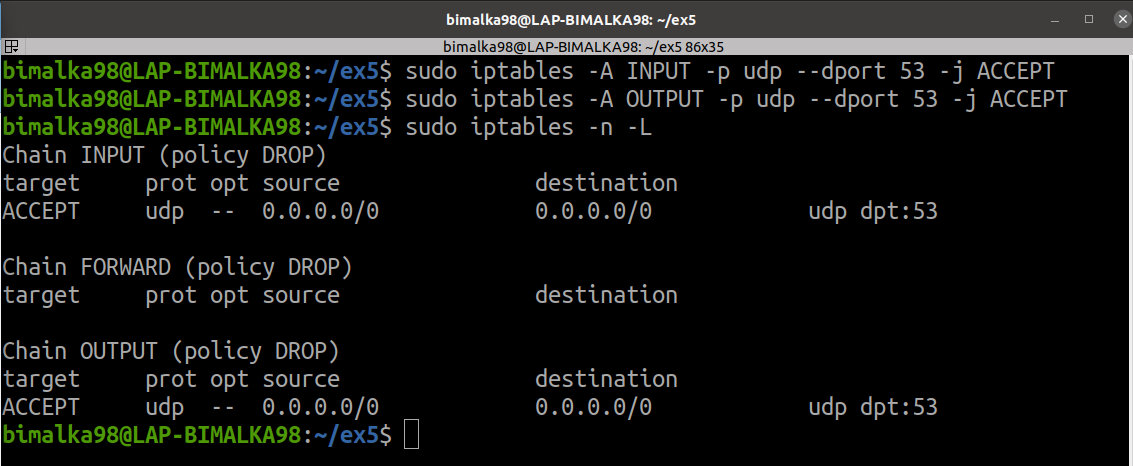
\includegraphics[width=0.65\columnwidth]{images/part1/6.png}
				\caption{Permitting input and output DNS traffic}
			\end{figure}
		\end{answer}
		
		\item Add iptables rules to accept local network incoming and outgoing traffic from the network 192.168.1.0/24. 
		\begin{answer}
			
			\begin{figure}[H]
				\centering
				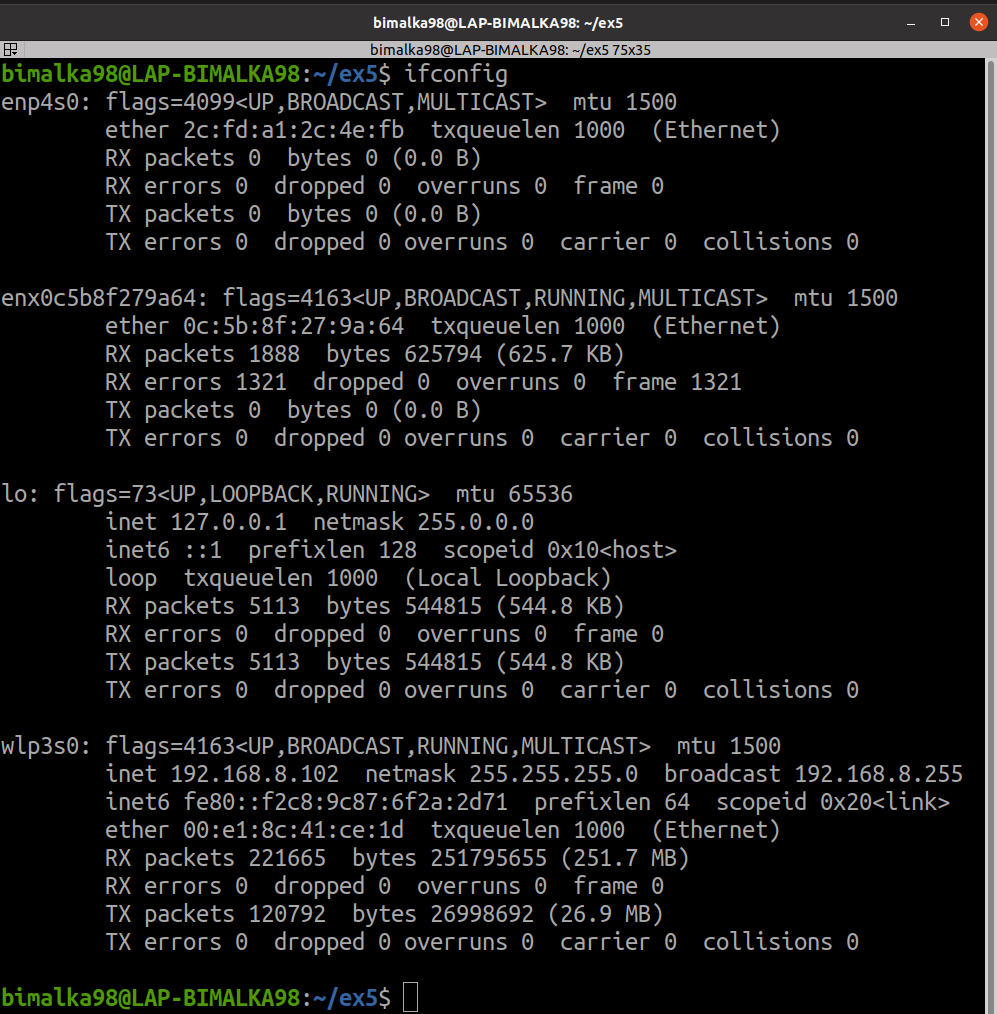
\includegraphics[width=0.65\columnwidth]{images/part1/ifconfig.png}
				\caption{Checking the CIDR of the current local network}
			\end{figure}
			
			\begin{figure}[H]
				\centering
				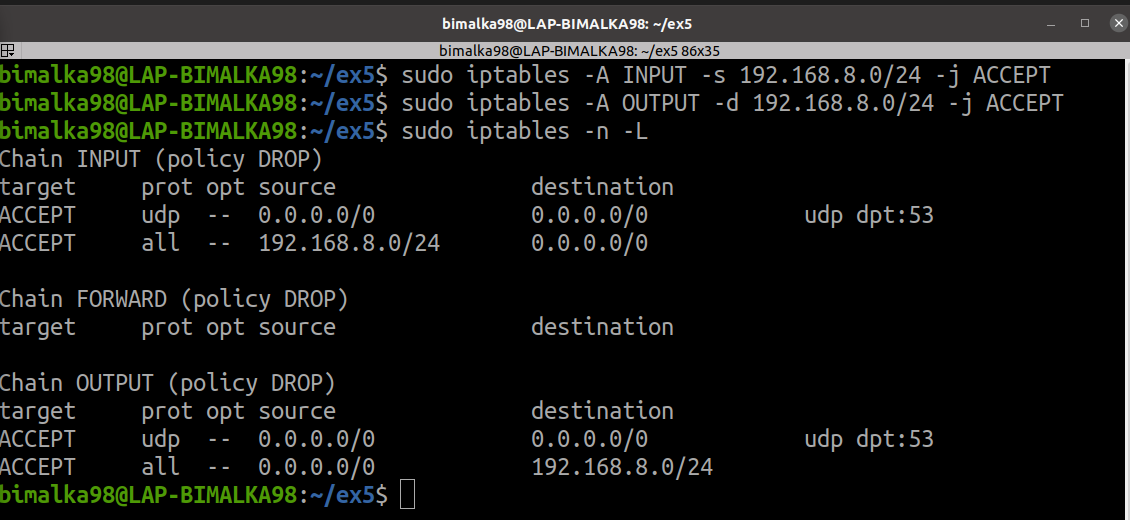
\includegraphics[width=0.65\columnwidth]{images/part1/7.png}
				\caption{Adding rules to accept local network incoming and outgoing traffic}
			\end{figure}
		\end{answer}
		
		\item Configure iptables rules to allow all HTTP traffic.
		\begin{answer}
			\begin{figure}[H]
				\centering
				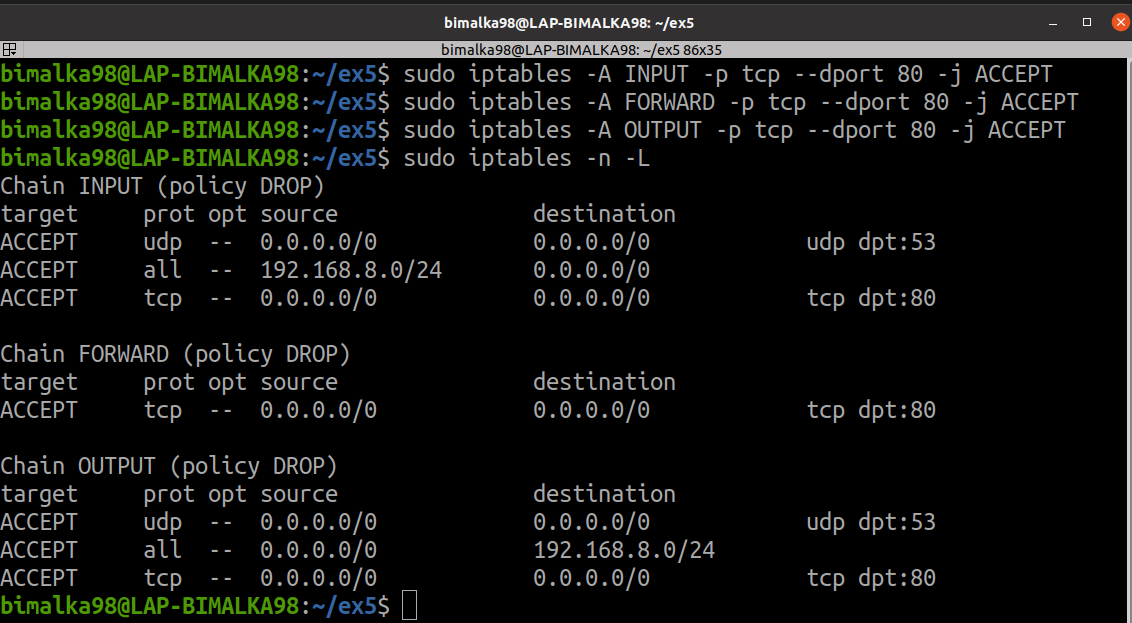
\includegraphics[width=0.65\columnwidth]{images/part1/8.png}
				\caption{Configuring rules to allow all HTTP traffic}
			\end{figure}
		\end{answer}
		
		\item View all iptables rules in your system and save them to a file \textbf{iptablesRuleNew.v4}. 
		\begin{answer}
			\begin{figure}[H]
				\centering
				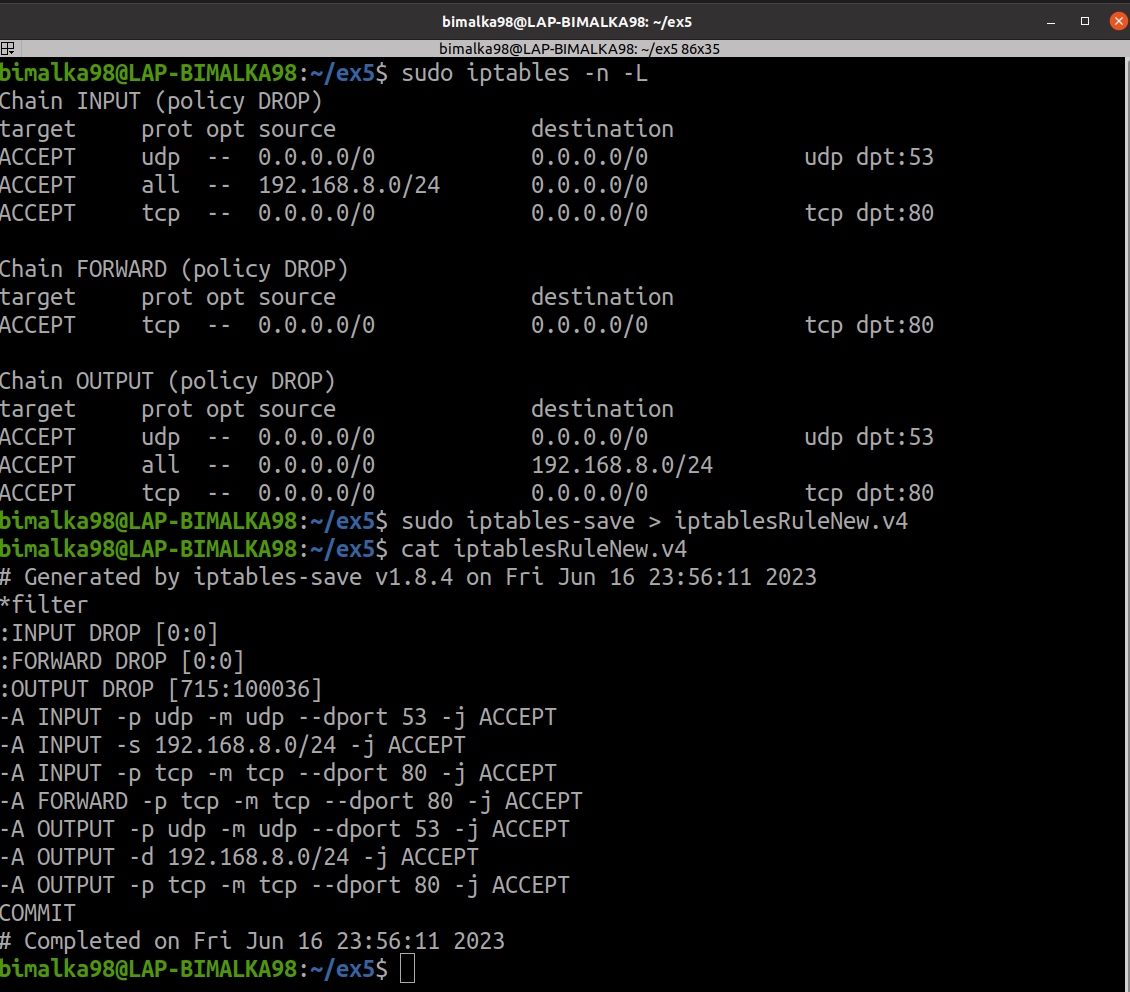
\includegraphics[width=0.65\columnwidth]{images/part1/9.png}
				\caption{Viewing all rules and saving them to a file}
			\end{figure}
		\end{answer}
		
		\item Create a file called \textbf{iptablesCommands.sh} and put all commands you ran from steps 4, 5 and 6 in the file. After creating the file, flush your iptables commands again and run \textbf{iptablesCommands.sh} file. View the iptables rules now and compare with the previous result.
		\begin{answer}
			\begin{figure}[H]
				\centering
				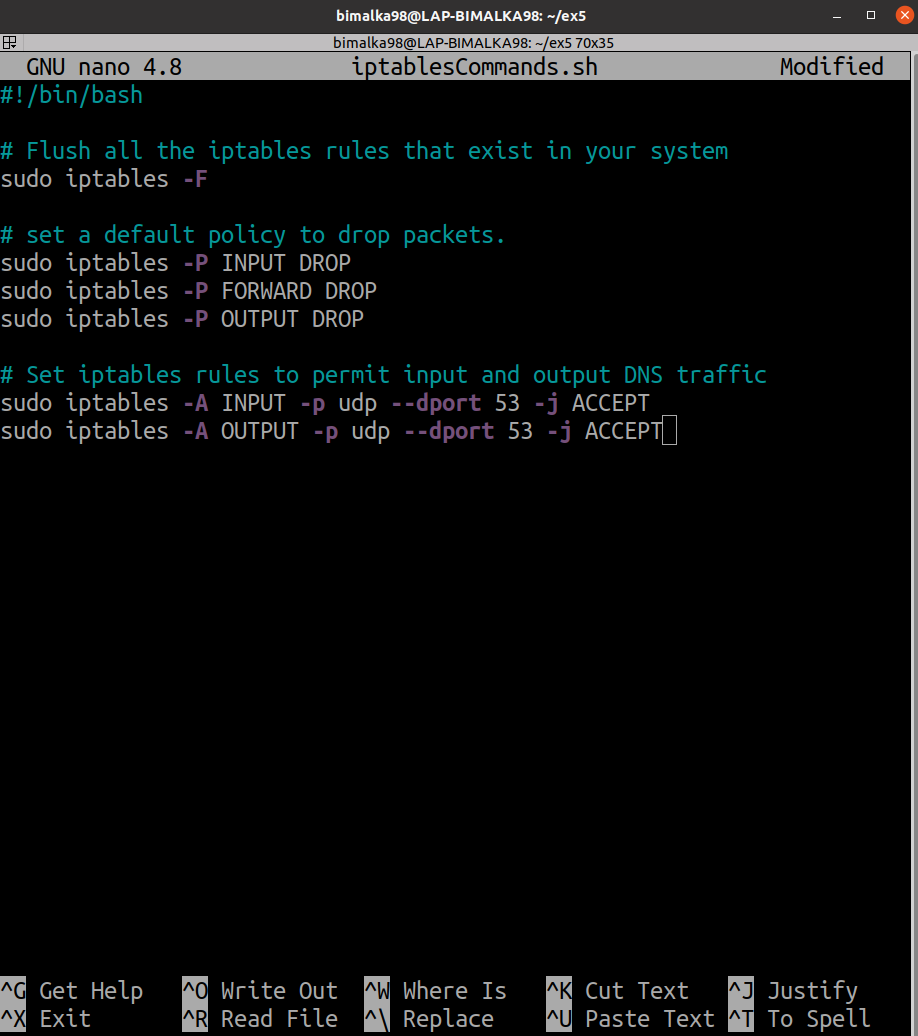
\includegraphics[width=0.65\columnwidth]{images/part1/10_1.png}
				\caption{Creating the shell script}
			\end{figure}
			
			\begin{figure}[H]
				\centering
				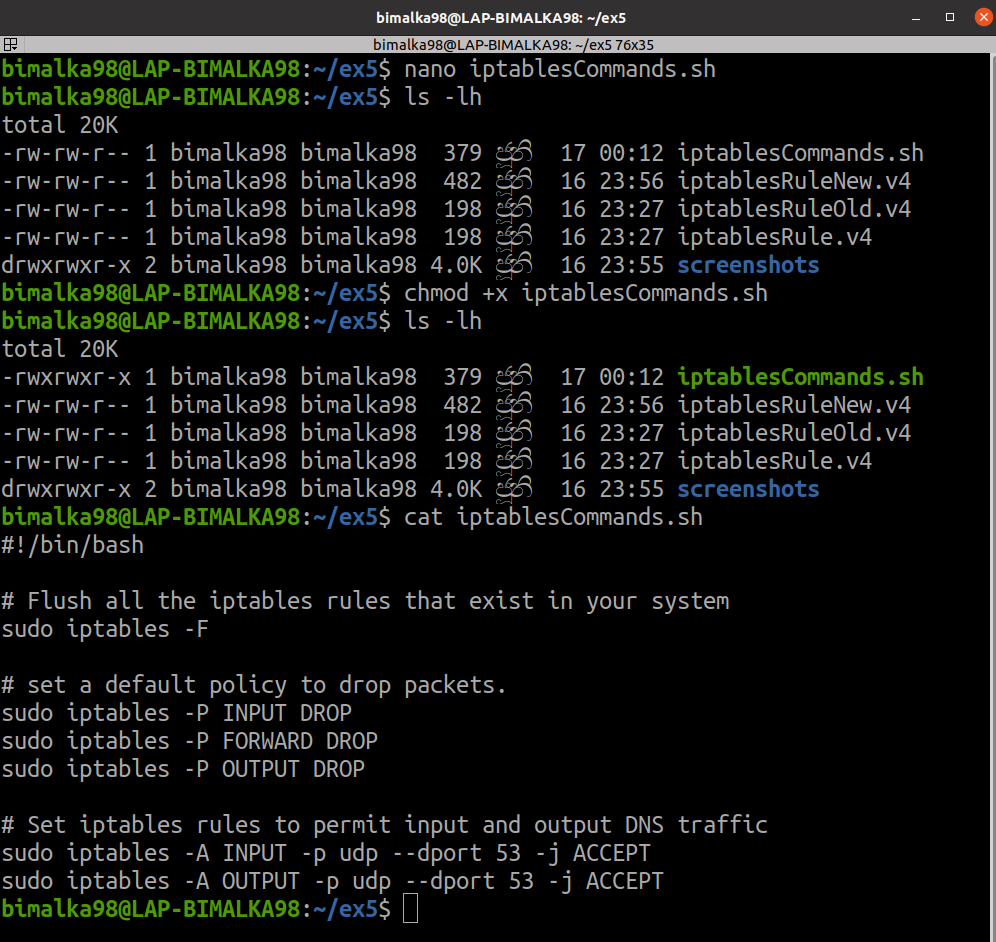
\includegraphics[width=0.65\columnwidth]{images/part1/10_2.png}
				\caption{Making the script executable}
			\end{figure}
		
			\begin{figure}[h]
				\centering
				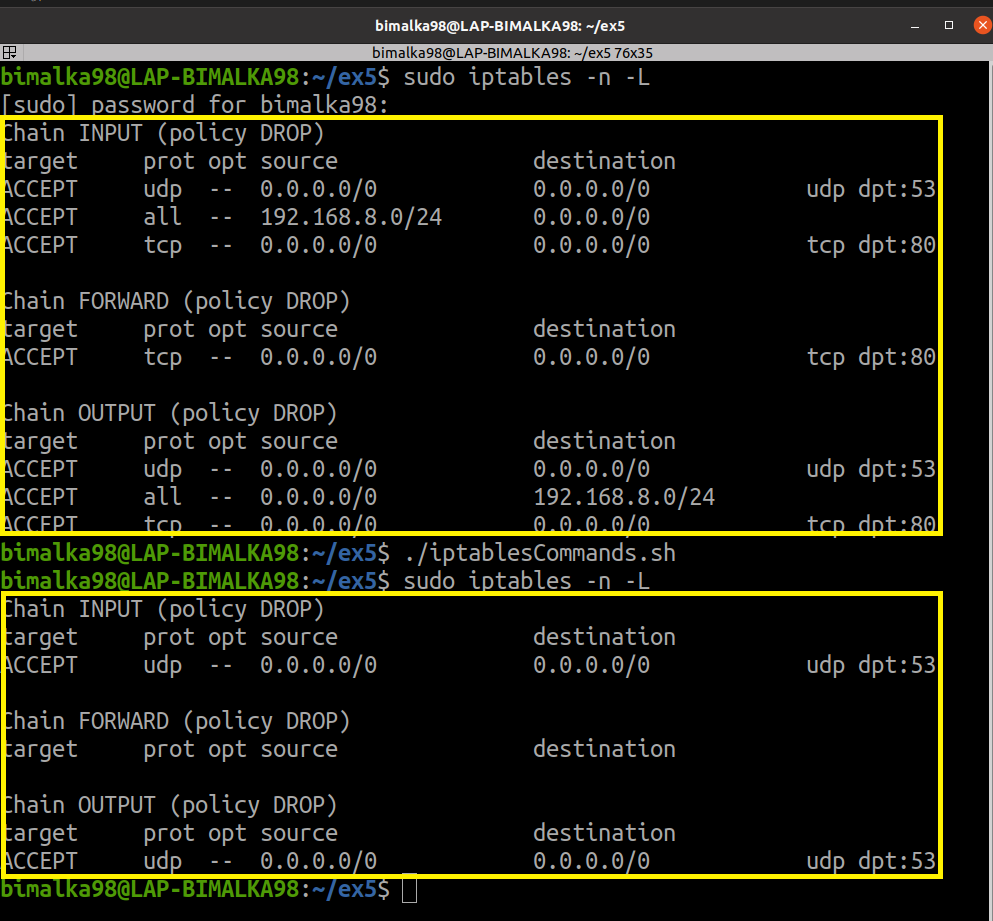
\includegraphics[width=0.65\columnwidth]{images/part1/10_3.png}
				\caption{Executing the shell script}
			\end{figure}
		\end{answer}
		
		\item Finally, flush your iptables rules again. But this time, load the saved iptables rules from the file \textbf{iptablesRuleNew.v4} using \texttt{iptables-restore} command. View the iptables rules and compare them with the ones you have in step 8.
		\begin{answer}
			\begin{figure}[h]
				\centering
				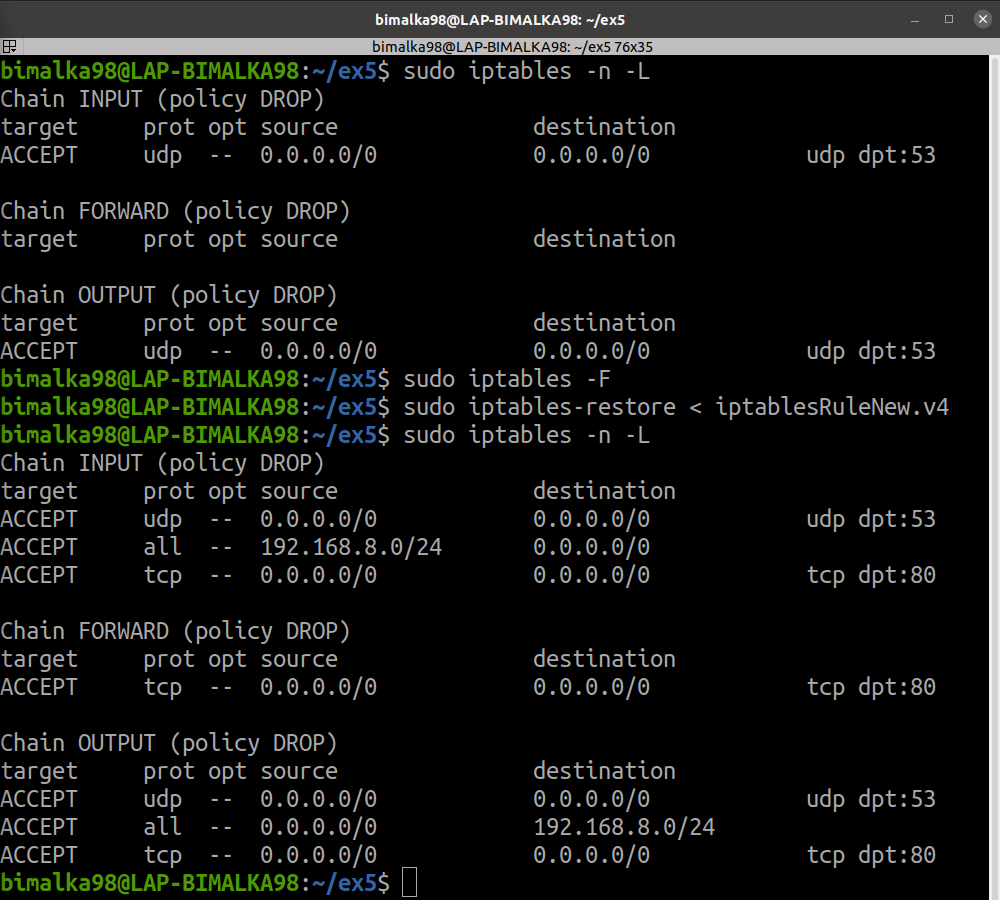
\includegraphics[width=0.65\columnwidth]{images/part1/11.png}
				\caption{Flushing current rules and restoring saved rules}
			\end{figure}
		\end{answer}
		
		\subsubsection*{Creating Firewall Rules with UFW}
		
		The scenario comprises of two virtual machines (VM1 IP - 192.168.46.140 and VM2 IP - 192.168.46.141) running on a host (HOST IP - 192.168.46.1) machine. VM1 is an Ubuntu virtual machine that has a firewall implemented/configured. 
		
		The current firewall ruleset is as below.
		\begin{figure}[H]
			\centering
			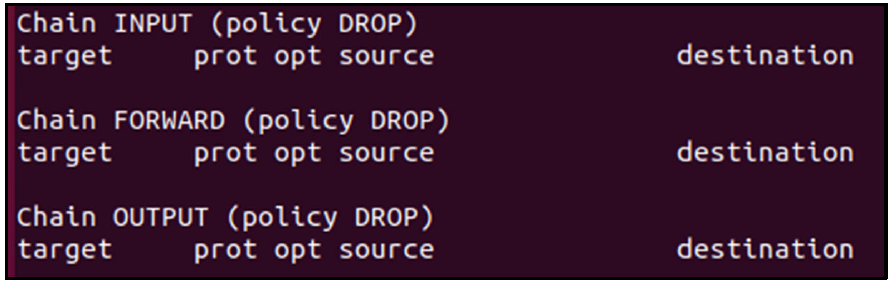
\includegraphics[width=0.5\columnwidth]{images/ex5-firewall-rules.png}
		\end{figure}
		
		All chain policies are set to drop traffic. To implement base rules, you can use the following commands:
		
		\begin{itemize}
			\item Delete any current rules associated with UFW using \texttt{sudo ufw reset}
			\item Disable UFW using \texttt{sudo ufw disable}
			\item Flush all iptables rules using \texttt{sudo iptables -F}
			\item Enable UFW using \texttt{sudo ufw enable}
			\item Deny outgoing traffic using \texttt{sudo ufw default deny outgoing}
		\end{itemize}
		
		\item Implement the following network administration in VM1:
		\begin{itemize}
			\item Access to VM1 from VM2 must only be allowed over FTP and Telnet.
			\item Access to VM1 from HOST must only be allowed over SSH
			\item Allow all outgoing traffic from VM1 with the exception of access to HTTP websites
		\end{itemize}
		
		In this task, you are asked to implement UFW rules on the ubuntu machine. You can pretend that VM2 and HOST exist in your network. List the commands you used to achieve the above. Add a screenshot of the terminal output after running the command \texttt{sudo ufw status numbered}.
		
		If the firewall is physically implemented, you could have tested the connections using PuTTY or the command line.
		
		\begin{answer}
			%% TODO: Add answer here
			Your answer here
		\end{answer}
		
		\subsubsection*{Scan systems with NMAP}
		In this section, you will scan for the Ports of a remote host. You will need to have two devices connected to the same local network to perform this task. 
		
		\item View ip addresses of both devices using \texttt{hostname -I} command.
		\begin{answer}
			%% TODO: Add answer here
			Your answer here
		\end{answer}
		\item Scan one host from the other host for TCP and UDP ports using \texttt{nmap} command.
		\begin{answer}
			%% TODO: Add answer here
			Your answer here
		\end{answer}\textbf{}
		
		\section*{Section 2}
		
		
		\item Briefly explain VLANs, VPNs, DMZs and Network Segmentation concepts outlining their similarities and differences.
		
		\begin{answer}
			%% TODO: Add answer here
			Your answer here
		\end{answer}
		
		\item Perform a comparison between IPsec and SSL.
		
		\begin{table}[htbp]
			\caption{Comparison of IPsec and SSL}
			\begin{tabularx}{\columnwidth}{|X|X|}
				\hline
				\textbf{IPsec} & \textbf{SSL}\\
				\hline
				\textcolor{blue}{Your answer here} & 
				\textcolor{blue}{Your answer here} \\ 
				\hline 
				\textcolor{blue}{Your answer here} & 
				\textcolor{blue}{Your answer here} \\ 
				\hline 
				
				
			\end{tabularx}
		\end{table}
		
		\item Explain the differences between an IDS, an IPS, and a firewall?
		
		\begin{answer}
			%% TODO: Add answer here
			Your answer here
		\end{answer}
		
		\item What is the difference between anomaly detection and signature or heuristic-based intrusion detection?
		
		\begin{answer}
			%% TODO: Add answer here
			Your answer here
		\end{answer}
		
	\end{enumerate}
	
\end{document}